\documentclass{article}
\usepackage{float}

\usepackage{amsmath}
\usepackage{amssymb}
\usepackage{graphicx}
\usepackage{inputenc}
\usepackage{hyperref}
\usepackage{listings}
\usepackage{polski}

\title{Raport}
\author{Łukasz Fabia}
\date{20.05.2024}

\begin{document}

\maketitle
\tableofcontents

\section{Wstęp}

\quad Celem badań jest analiza danych dotyczących ofert pracy w IT. W swojej pracy postaram się
odpowiedzieć na pytanie, jakie są najbardziej poszukiwane umiejętności w branży IT oraz ile można zarobić
znając dane języki, frameworki czy narzędzia. W tym celu postram się wykorzystać sci-kit learn do stworzenia
modelu regresji liniowej, który pozwoli mi przewidzieć zarobki na podstawie umiejętności (technologii).


\section{Dane}

\quad Dane pozyskam z serwisu \href{https://justjoin.it/}{justjoin.it}, który zbiera oferty pracy z wielu różnych serwisów, zatem
ofert pracy będzie całkiem sporo. Na stronie mamy katergorie, które mogą być przydatne do analizy, takie jak:
JS, PHP, Ruby, Python, Java, Net, Mobile, C, DevOps, Security, Data, Go, Game, Scala. W mojej analizie skupię się na nich.
\quad Dodatkowo analizuję zarobki tylko na b2b oraz na umowie o prace (uop), ponieważ są to najbardziej popularne formy zatrudnienia w IT a inne formy takie jak umowa
o zlecenie czy umowa o staż pratykcznie nie występują. Do analizy będę również brał pod uwagę lokalizację.

\textbf{\newline Technologia} - język programowania, framework, narzędzie, które jest wymagane w ofercie pracy.

\subsection{Model danej}
\quad Dane będą zawierały informacje o ofertach pracy, takie jak:
\begin{itemize}
    \item tytuł oferty
    \item widełki dla B2B
    \item widełki dla UOP
    \item technologie dotyczące umowy
    \item lokalizacja
    \item doświadczenie {junior, mid, senior}
    \item typ pracy {stacjonarnie, hybrydowo, zdalnie}
\end{itemize}

\subsection{Obsługa technologii, lokalizacji}

\quad Najpierw zdefiniuje sobie słownik klucz, wartość, gdzie klucz to ustandaryzowana technologia, a wartość do synonimy tej technologii.

\textit{np. \ "JavaScript": [
"javascript",
"js",
"node.js",
"nodejs",
"express.js",
"expressjs",
],}

\quad Dzięki temu będę mógł przekonwertować technologie z oferty pracy na wektor binarny, gdzie 1 oznacza, że technologia jest wymagana, a 0, że nie jest wymagana. Kolejnym
krokiem będzie obsługa lokalizacji. W tym przypadku jeśli oferta dot. kilku miast to znaczy, że pojawi się w zbiorze
klika ofert z tymi samymi danymi, ale dla różnych miast.


\subsection{Pozykiwanie danych}

\quad Dane będą pozyskiwane z ww. serwisu, za pomocą narzędzi do web scrappingu w moim przypadku będzie
to \texttt{Selenium}, ponieważ strona ma dynamicznie ładowany content.


Kroki:
\begin{itemize}
    \item napisanie skryptu pobierającego linki do ofert pracy z danej kategorii, ponieważ nie chcemy śmiecowych ofert typu Product manager
    \item napisanie skryptu przetwarzającego linki do ofert pracy, aby pobrać dane z oferty
    \item przekierowanie wyniku do pliku json.
    \item normalizacja oraz oczyszczanie danych, kodowanie technologii, do wektora przy pomocy MultiLabelBinarizer z \texttt{sklearn}
    \item kodowanie duplkacja ofert z różnymi lokalizacjami oraz kodowanie typu pracy i doświadczenia (\texttt{label encoding})
    \item usunięcie ofert z wynagrodzniem godzinowym bo zalezą one od ilości przepracowanych godzin
\end{itemize}

\textit{Ofert ze stawką godzinową było kilka więc nie wypływają one na wyniki.}

\section{Wygląd do danych}

\textit{uwaga przykładowe dane nie zawierają wszystkich kolumn bo jest ich za dużo, wszystkie dane można znaleźć w ../data/jobs.csv}


\textbf{Przykładowe dane:}


\begin{table}[h]
    \centering
    \begin{tabular}{|c|c|c|c|c|}
        \hline
        \multicolumn{1}{|c|}{\textbf{title}} & \textbf{min\_b2b} & \textbf{max\_b2b} & \textbf{min\_uop} & \textbf{max\_uop} \\ \hline
        Senior Software Engineer             & 0.0               & 0.0               & 18000.0           & 28000.0           \\ \hline
        Senior Backend Node.js Engineer      & 0.0               & 0.0               & 18360.0           & 25125.0           \\ \hline
        Senior Fullstack Developer           & 22680.0           & 27216.0           & 16600.0           & 19920.0           \\ \hline
    \end{tabular}
\end{table}


\begin{table}[h]
    \centering
    \begin{tabular}{|c|c|c|c|}
        \hline
        \textbf{location\_code} & \textbf{operating\_mode\_code} & \textbf{experience\_code} \\ \hline
        38                      & 0                              & 2                         \\ \hline
        17                      & 2                              & 2                         \\ \hline
        51                      & 0                              & 2                         \\ \hline
    \end{tabular}
\end{table}


\begin{table}[h]
    \centering
    \begin{tabular}{|c|c|c|c|}
        \hline
        \textbf{AWS} & \textbf{JavaScript} & \textbf{React} & \textbf{Java} \\ \hline
        1            & 1                   & 1              & 0             \\ \hline
        0            & 1                   & 1              & 0             \\ \hline
        1            & 1                   & 1              & 0             \\ \hline
    \end{tabular}
\end{table}

\newpage

\section{Rozkłady i statystyki}

\quad Aktualnie w zbiorze \textit{jobs.csv} znajduje się \textbf{4574} ofert pracy, które będą poddane
analizie. Wszystkie dane są znormalizowane i gotowe do analizy. Analizę można zacząć od średniej zarobków
dla kontraktu B2B oraz UOP.


\textbf{Widełki dla Juniora: }

\begin{table}[h]
    \centering
    \begin{tabular}{|c|c|c|c|}
        \hline
        \textbf{PLN}             & \textbf{B2B} & \textbf{UOP} \\ \hline
        \textbf{średnie widełki} & 8555.40      & 13558.71     \\ \hline
        \textbf{min widełki}     & 4250.00      & 6000.00      \\ \hline
        \textbf{max widełki}     & 16443.00     & 28000.00     \\ \hline
    \end{tabular}
    \caption{Średnie zarobki w PLN dla \texttt{juniora} w Polsce}
\end{table}

\textbf{Widełki dla Mida: }

\begin{table}[h]
    \centering
    \begin{tabular}{|c|c|c|c|}
        \hline
        \textbf{PLN}             & \textbf{B2B} & \textbf{UOP} \\ \hline
        \textbf{średnie widełki} & 12378.99     & 18041.77     \\ \hline
        \textbf{min widełki}     & 5000.00      & 7000.00      \\ \hline
        \textbf{max widełki}     & 25000.00     & 30000.00     \\ \hline
    \end{tabular}
    \caption{Średnie zarobki w PLN dla \texttt{mida} w Polsce}
\end{table}

\textbf{Widełki dla Seniora: }

\begin{table}[h]
    \centering
    \begin{tabular}{|c|c|c|c|}
        \hline
        \textbf{PLN}             & \textbf{B2B} & \textbf{UOP} \\ \hline
        \textbf{średnie widełki} & 18930.61     & 25848.46     \\ \hline
        \textbf{min widełki}     & 8000.00      & 11000.00     \\ \hline
        \textbf{max widełki}     & 40000.00     & 80000.00     \\ \hline
    \end{tabular}
    \caption{Średnie zarobki w PLN dla \texttt{seniora} w Polsce}
\end{table}
\newpage
\subsection{Jak się pracuje w IT?}

\begin{figure}[H]
    \centering
    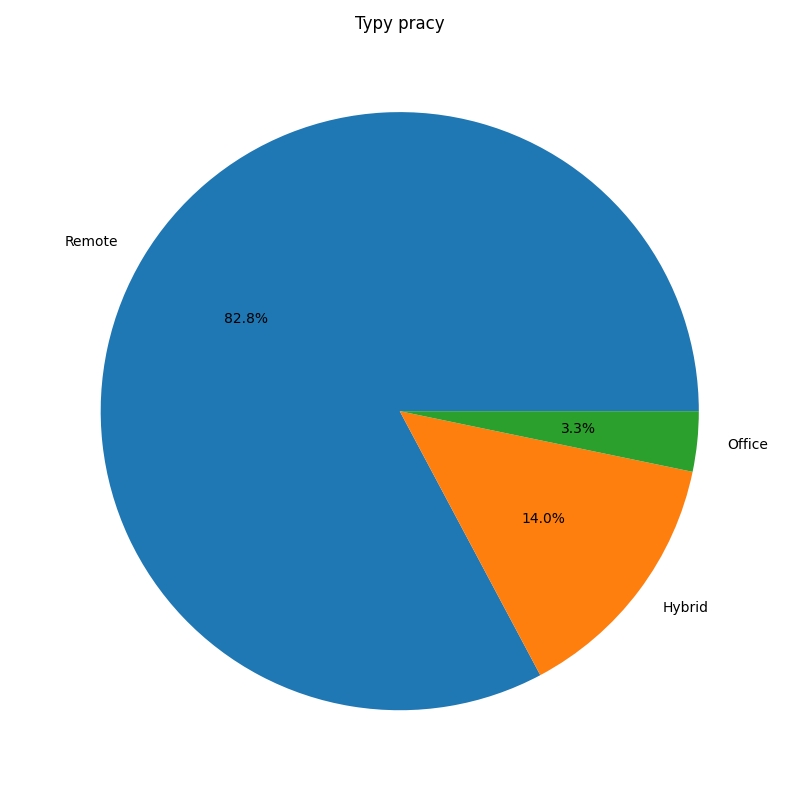
\includegraphics[width=0.8\textwidth]{../analysis/plots/rozkłady/typy_pracy.png}
    \caption{Rozkład typów pracy}
\end{figure}

\quad Jak widać najwięcej ofert pracy dotyczy pracy zdalnej.


\subsection{Kogo szukają pracodawcy?}

\begin{figure}[H]
    \centering
    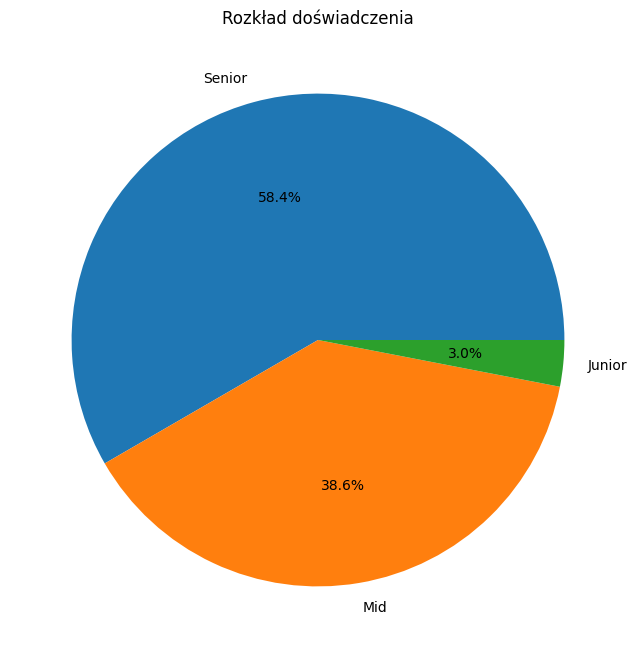
\includegraphics[width=0.8\textwidth]{../analysis/plots/rozkłady/doświadczenie.png}
    \caption{Rozkład typów pracy}
\end{figure}

\quad Tak jak można było się spodziewać - najwięcej ofert pracy jest dla seniorów,
stąd też wynika dlaczego tak dużo kontraktów dotyczy pracy zdalnej. Chociaż
warto powiedzieć sytuacja midów jest również dobra. Gorzej jest z ofertami dla młodych programistów.
Tutaj liczba ofert wyniosła zaledwie 139, co jest bardzo małą liczbą w porównaniu do innych grup.

\textit{Czy to oznacza, że młodzi programiści mają trudniej, a słynne "eldorado" w IT jest tylko dla doświadczonych programistów?}

\quad Tutaj można powiedzieć, że juniorzy mają trudniej \textbf{wejść} do branży, ale zarobki po wejściu są naprawdę atrakcyjne,
no, ale tutaj problem może być z wejściem.


\subsection{Jak rozkładają się zarobki?}

\begin{figure}[H]
    \centering
    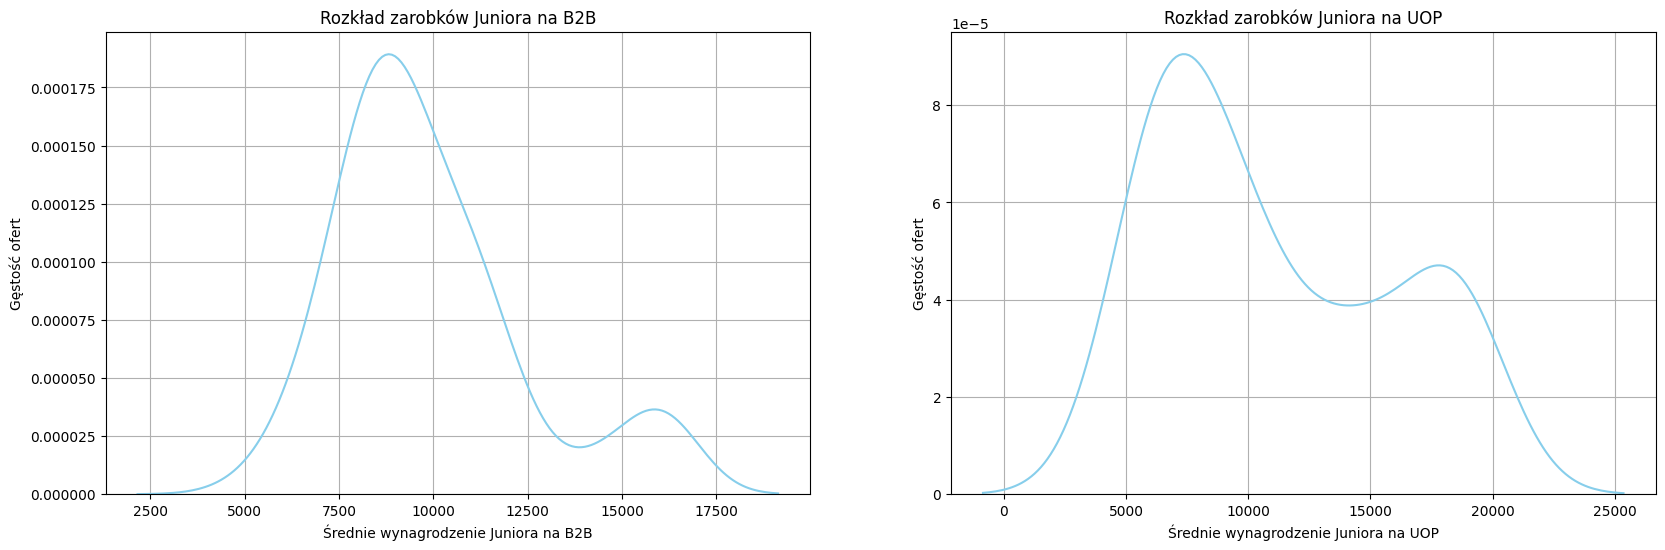
\includegraphics[width=0.8\textwidth]{../analysis/plots/rozkłady/b2b_uop_junior.png}
    \caption{Rozkłady zarobków dla poszczególnych umów dla juniorów}
\end{figure}

\begin{figure}[H]
    \centering
    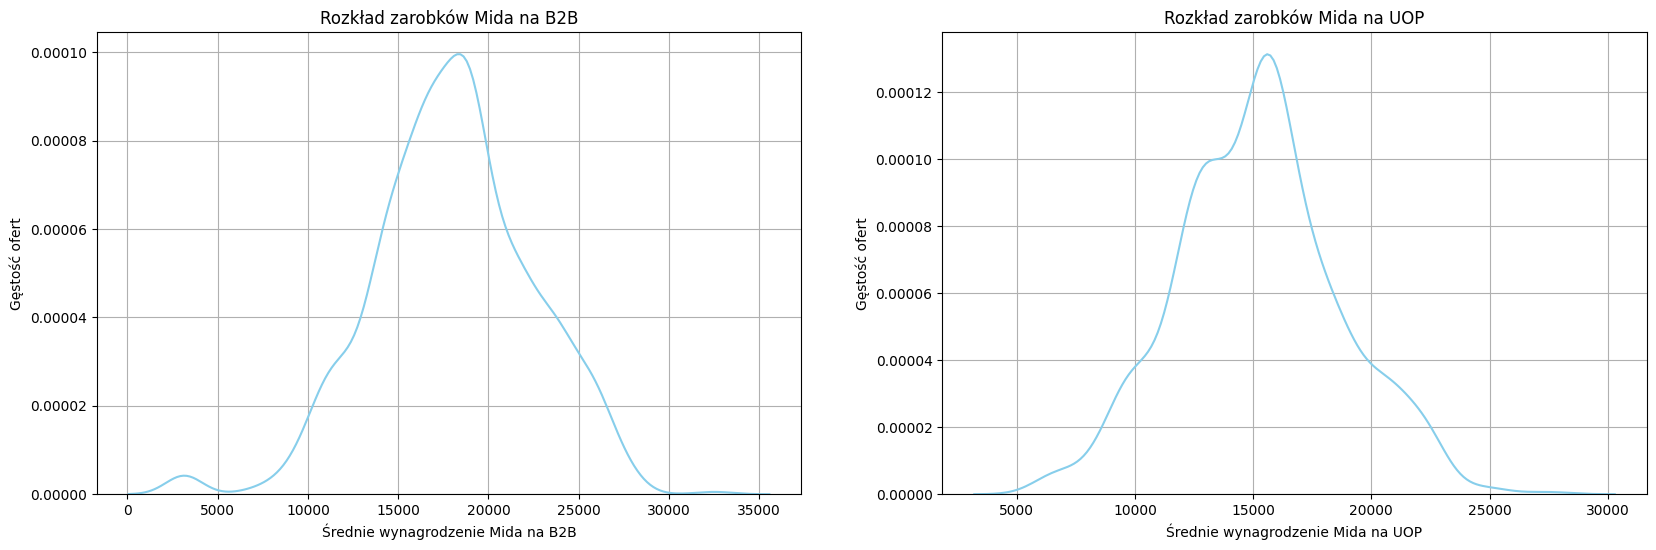
\includegraphics[width=0.8\textwidth]{../analysis/plots/rozkłady/b2b_uop_mid.png}
    \caption{Rozkłady zarobków dla poszczególnych umów dla midów}
\end{figure}

\begin{figure}[H]
    \centering
    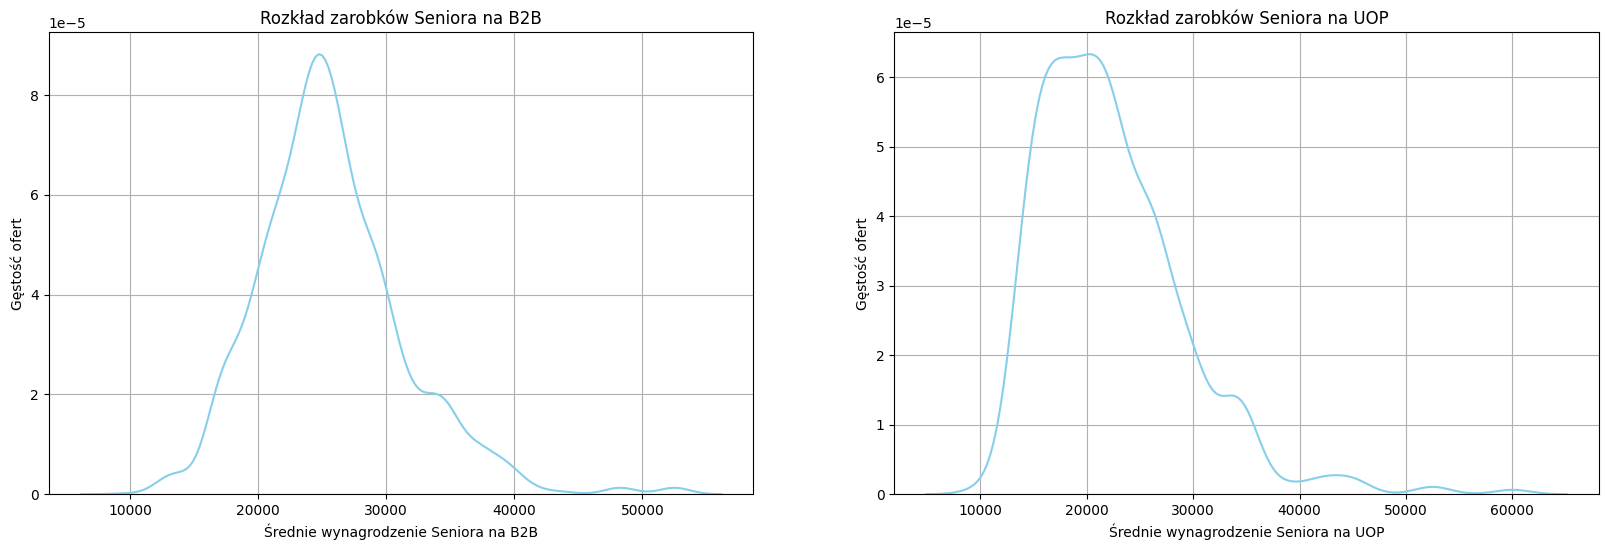
\includegraphics[width=0.8\textwidth]{../analysis/plots/rozkłady/b2b_uop_senior.png}
    \caption{Rozkłady zarobków dla poszczególnych umów dla seniorów}
\end{figure}


\subsection{Jakie technologie są najbardziej poszukiwane?}

\begin{figure}[H]
    \centering
    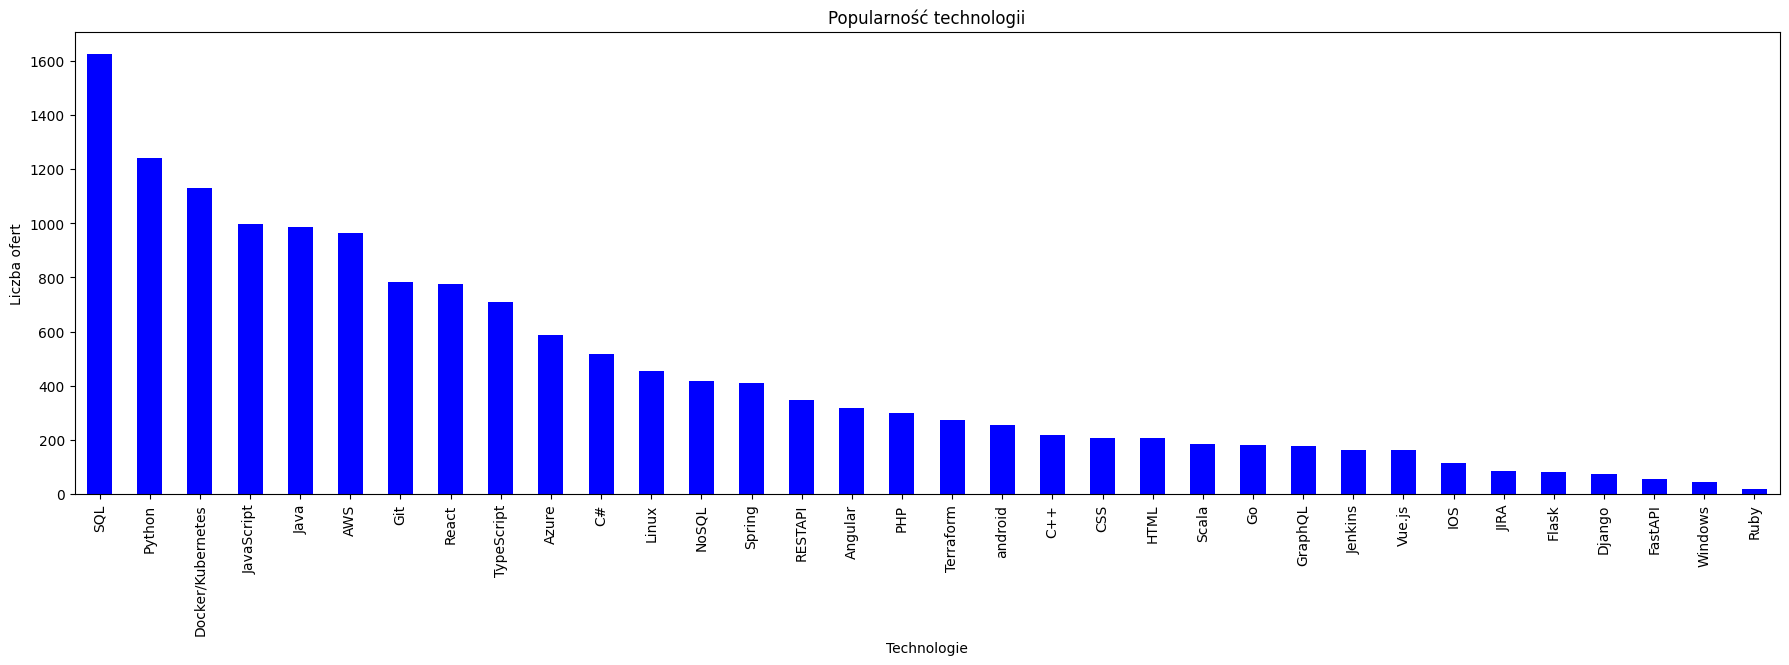
\includegraphics[width=0.8\textwidth]{../analysis/plots/rozkłady/technologie.png}
    \caption{Popularne technologie w ofertach pracy w Polsce}
\end{figure}

\quad Tutaj moim zdaniem troche zaskoczenie ponieważ bez \texttt{SQL} ciężko znaleźć prace w IT, czyli
bazy danych to jest podstawa przy rekrutowanu się do pracy. Oczywiście nie mogło zabraknąć \texttt{Pythona} oraz \texttt{JavaScriptu} jeśli chodzi o języki skryptowe.
Co warto zazanczyć narzędzia takie jak \texttt{Docker} czy \texttt{Kubernetes} również są bardzo popularne i warto je znać. \texttt{Java} wygrywa z \texttt{C\#} a \texttt{GNU/Linux} deklasuje \texttt{Windowsa}.


\subsection{Gdzie jest największy popyt na programistów?}

\begin{figure}[H]
    \centering
    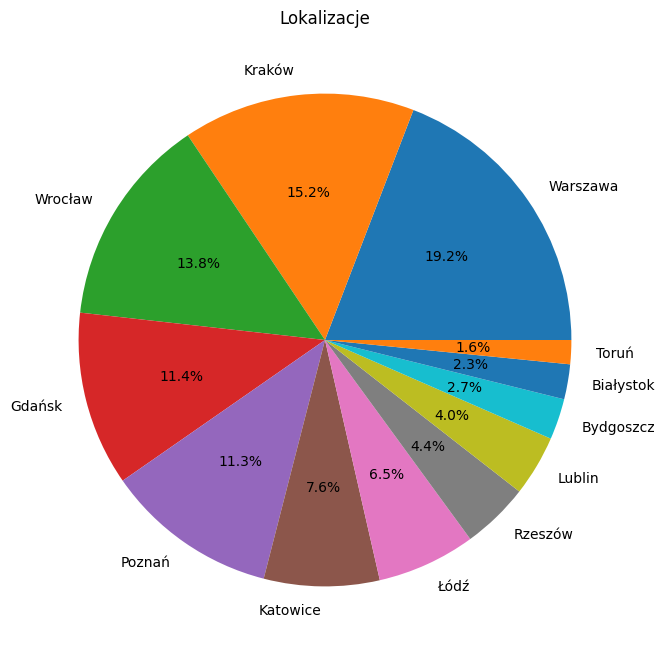
\includegraphics[width=0.8\textwidth]{../analysis/plots/rozkłady/lokalizacje.png}
    \caption{Popularne miasta w ofertach pracy w Polsce}
\end{figure}

\quad Zestawienie miast jest zgodne z oczekiwaniami, najwięcej ofert pracy jest kolejno w \textbf{Warszawie}, \textbf{Krakowie} oraz \textbf{Wrocławiu}, chociaż
\textbf{Gdańsk} również pojawiał się w dużej ilości ofert pracy.


\subsection{Gdzie poszukiwani są juniorzy?}

\begin{figure}[H]
    \centering
    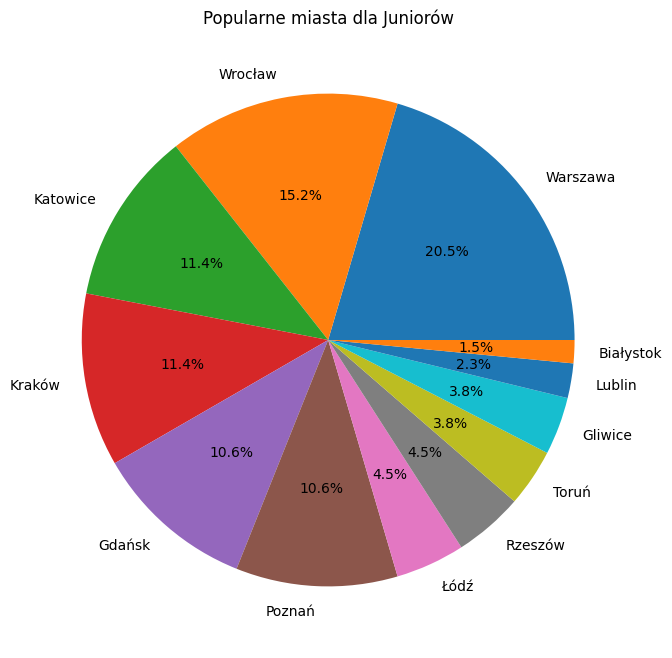
\includegraphics[width=0.8\textwidth]{../analysis/plots/rozkłady/lokalizacje_dla_juniorów.png}
    \caption{Popularne miasta w ofertach dla juniorów}
\end{figure}

\quad \textbf{Warszawa} jest najbardziej przyjazna dla juniorów, ale
warto zauważyć, że wykres nie różni się bardzo od poprzedniego z jednym, \textit{ale} - \textbf{Katowice} są
na 3 miejscu w zestawieniu dla juniorów, co może być zaskoczeniem.


\section{Powiązania między danymi}

\subsection{Powiązania między technologiami}

\begin{figure}[H]
    \centering
    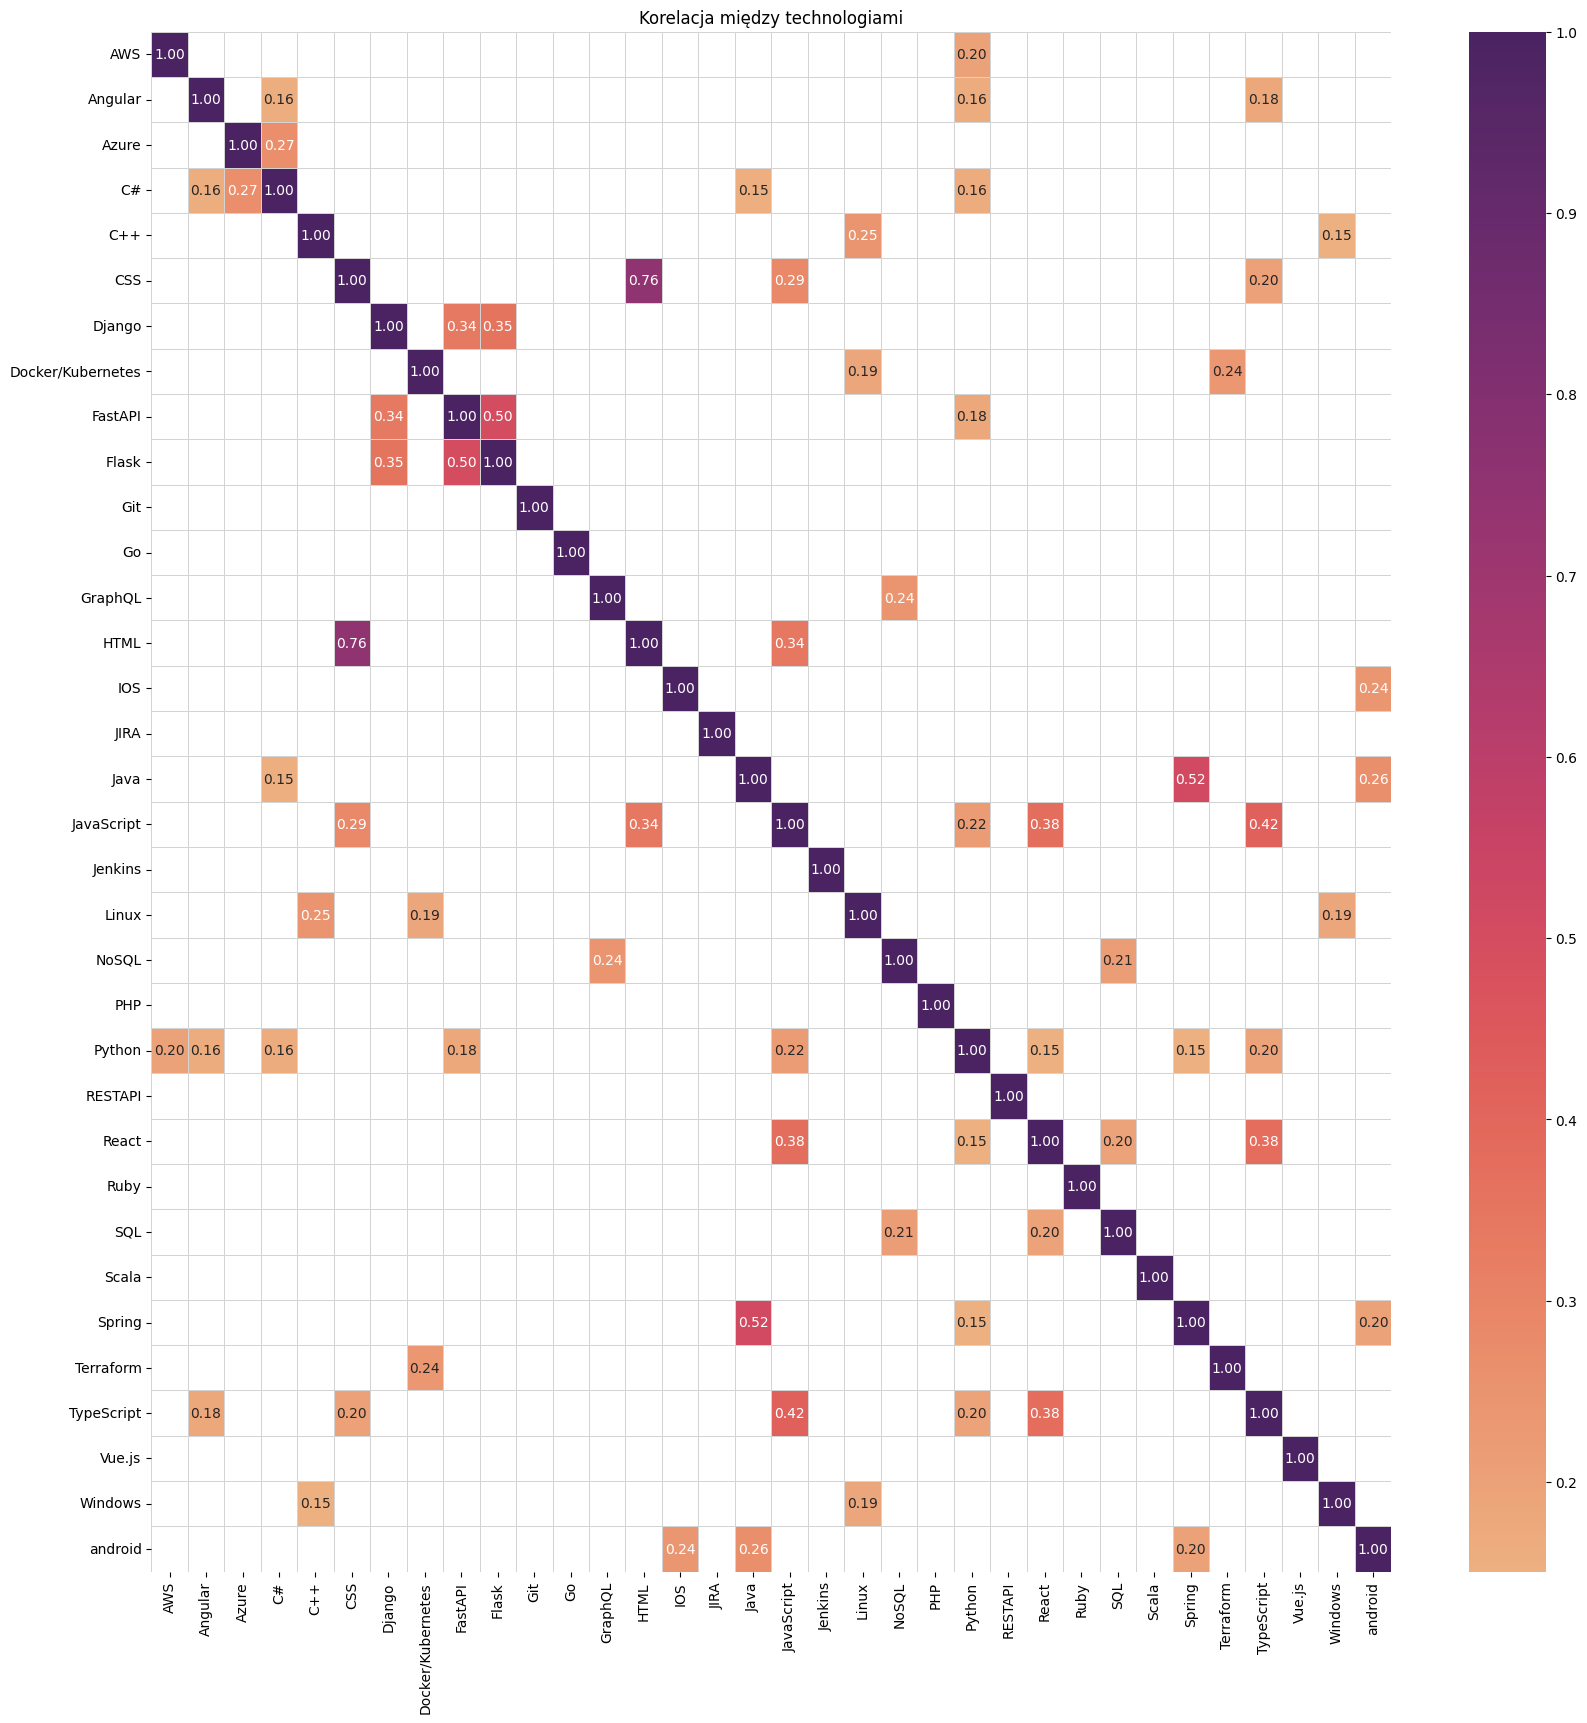
\includegraphics[width=0.8\textwidth]{../analysis/plots/korelacje/powiązania_technologii.png}
    \caption{Powiązania między technologiami, zawierająca tylko wartości korelacji większe niż 0.14}
\end{figure}

\quad \textbf{Co można zauważyć?}

\begin{enumerate}
    \item HTML i CSS idą ze prawie w parze - co jest zrozumiałe, bo to podstawy front-endu
    \item Przy Javie warto znać Springa
    \item React i JS i TS często pojawiają sie razem w ofertach pracy obok HTML i CSS
    \item Jak sie uczy Django to warto znać inne frameworki backendowe takie jak Flask czy FastAPI
    \item Jak sie idzie w Embedded to warto znać C/C++ oraz Linux
\end{enumerate}

\quad To tylko kilka przykładów wymienionych wynikający z obrazka powyżej, ale warto zauważyć, że nie ma tutaj dużo
powiązań między technologiami, co może wynikać z tego, że technologie są zbyt różne, aby były powiązane.


\subsection{Powiązania między innymi zmiennymi}

\begin{figure}[H]
    \centering
    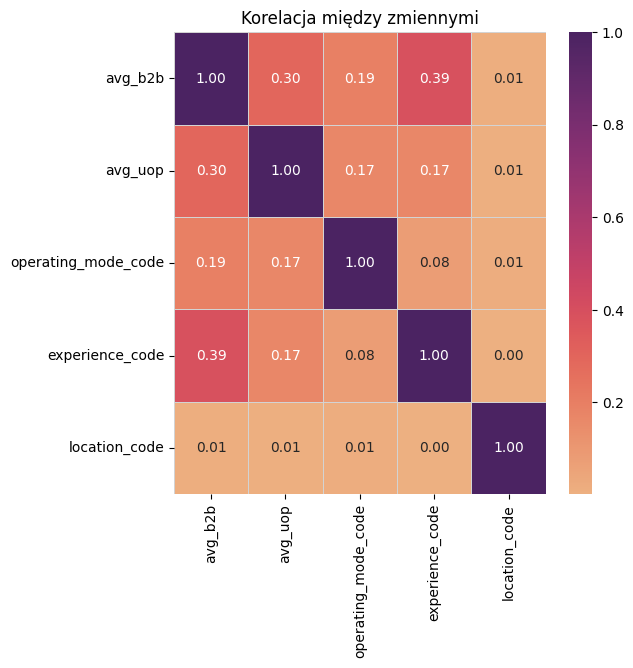
\includegraphics[width=0.8\textwidth]{../analysis/plots/korelacje/inne_zmienne.png}
    \caption{Powiązania między innymi zmiennymi}
\end{figure}

\quad \textbf{Co można zauważyć?}

\begin{enumerate}
    \item W jakiś spobób powiązane są ze sobą zarobki na B2B i UOP - ma sens
    \item Wynagrodzenie na B2B i UOP jest powiązane z doświadczeniem
\end{enumerate}


\subsection{Zarobek a technologie}

\begin{figure}[H]
    \centering
    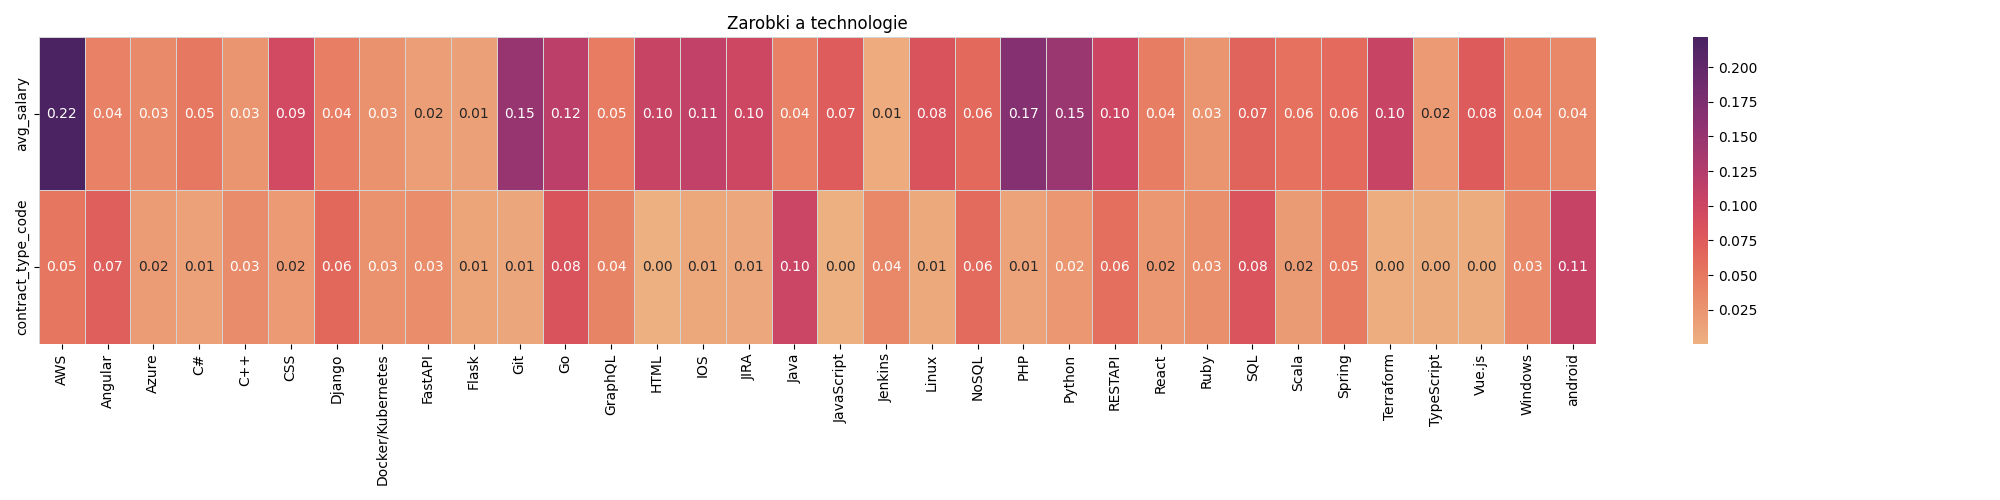
\includegraphics[width=\textwidth]{../analysis/plots/korelacje/zarobki_a_technologie.png}
    \caption{Powiązania między zarobkiem a technologiami}
\end{figure}

\quad Tutaj jest kilka ciekawych powiązań, które warto zauważyć, np. na umowie o prace znaczenie ma
znajomość: Go, AWS, Angulara, Java, SQL czy Andorida, chociaż nie są to mocne powiązania. Natomiast na B2B nie ma jakiś znaczących powiązań można wskazać
np. Resta, AWS, Docker/Kubernetes czy PHP, ale są to watości rzędu 0.09, co nie jest imponującym wynikiem.


\end{document}


